\documentclass{article}

\usepackage{fullpage}
\usepackage[english]{babel}
\usepackage[utf8x]{inputenc}
\usepackage{amssymb}
\usepackage{graphicx}
\usepackage[colorinlistoftodos]{todonotes}
%\usepackage[]{algorithm2e}
\usepackage{enumerate,url}
\usepackage{hyperref}
\hypersetup{colorlinks=true}
\usepackage{enumitem}
\usepackage{tcolorbox}
\usepackage[noline,noend]{algorithm2e}
\usepackage{amsmath}
%\usepackage{pythontex}
\usepackage{pythonhighlight}
\SetNlSty{}{}{}

\let\oldnl\nl% Store \nl in \oldnl
\newcommand\nonl{%
  \renewcommand{\nl}{\let\nl\oldnl}}% Remove line number for one line

\title{CSE 6140 / CX 4140 Assignment 2\\due Oct 2, 2020 at 11:59pm on Canvas }
\author{Shasha Liao}
\date{}
\begin{document}
\maketitle

\noindent\fbox{\parbox{\dimexpr\textwidth-2\fboxsep-2\fboxrule\relax}{
\vspace{2mm}
Please upload two files: 
\begin{enumerate}
 \item a single PDF named \texttt{assignment.pdf} containing your solutions for Problems 1 and 2; and a report for Problem 3.
 \item a single zip file named \texttt{code.zip} containing your code,
     README, and results for Problem 3
\end{enumerate}
}}

\section{Dynamic Programming: Atlanta MARTA [13 pts]}
The  Metropolitan  Atlanta  Rapid Transit  Authority  (MARTA) is  the  principal  public  transportoperator in the Atlanta metropolitan area. It was Formed in 1971 as strictly a bus system, and today, it is transporting almost 450,000 passengers a day (bus and train). Currently, MARTA Passes are the cheapest option for those who regularly use MARTA for transportation. Assume the MARTA Passes are sold in three following forms:

\begin{itemize}
\item Daily: A 1-day pass sold for $tickets[0]$ dollars;
\item Weekly: A 7-day pass sold for $tickets[1]$ dollars;
\item Monthly: A 30-day pass sold for $tickets[2]$ dollars.
\end{itemize}

For instance, $tickets = {2, 7, 20}$ means we need to pay $\$2$, $\$7$, and $\$20$ for each daily, weekly,and monthly pass, respectively. The passes allow consecutive days of travel.  For example, if we get a weekly pass on day 5, then we can travel for 7 consecutive days which are: day 5, 6, 7, 8, 9,10, and 11. George P. Burdell is a student at Georgia Tech and he has already organized his commuting plan for  the  upcoming  year.  In  his  plan,  each   day of  year  is  specified   by an  integer   identification number from 1 to 365. Therefore, he can represent his commuting plan as an array of integers. For instance, days = {8, 9, 10, 11, 14, 17, 18, ...} means George needs to commute to the school on the 8th, 9th, 10th, 11th, ... days of year. He asked you to help him find the minimum amount of money that he should spend to purchase MARTA Passes for commuting to school in the next year. 

\begin{itemize}

\item[a)] (3 pts) Prove the optimal substructure.
\begin{tcolorbox}
\textbf{Solution:} \\
\textbf{Goal:}  calculate the minimum amount of money that George should spend to purchase MARTA Passes according to his commuting plan for $n = 365$ days in the next year. Denote that value by $OPT(n)$. \\
\textbf{Define subproblem:}  calculate the minimum amount of money he should spend by optimal solution for the first $j$ days in the next year $OPT(j)$. \\

Consider an optimal solution O for the days $\{1, 2, ..., j\}$. On day $j$, there are two possible cases for George's commuting plan.
\begin{itemize}
\item \textbf{Case 1}: George dose not plan to commute  on day $j$. Then $OPT(j) = OPT(j-1)$
\item \textbf{Case 2}: George plans to commute on day $j$. Then he has three options:
\begin{itemize}
\item \textbf{Option 1}: George uses a daily pass to take MARTA on day $j$. 
\item \textbf{Option 2}: George uses a weekly pass (expiring on day $j$) to take MARTA on day $j$.
\item \textbf{Option 3}: George uses a monthly pass (expiring on day $j$) to take MARTA on day $j$.
\end{itemize}

Now we are going to show that for each option we can calculate $OPT(j)$ from $OPT(k)$ where $k < j$.\\
\begin{itemize}
\item \textbf{Option 1}: $OPT(j) = OPT(j - 1) + tickets[0]$ since George has to purchase a daily pass on day $j$.
\item \textbf{Option 2}: $OPT(j) = OPT(j - 7) + tickets[1]$ since George has to purchase a weekly pass on day $j - 6$.
\item \textbf{Option 3}: $OPT(j) = OPT(j - 30) + tickets[2]$ since George has to purchase a monthly pass on day $j - 29$.
\end{itemize}
So in this case, $$OPT(j) = \min \{ OPT(j - 1) + tickets[0],  OPT(j - 7) + tickets[1], OPT(j - 30) + tickets[2]\}.$$
\end{itemize}
So we will have the recursive relation presented in part b). Now we prove that this algorithm computes correctly the optimal value
for each $j = 0, 1, 2, ..., n$ by induction. 
\begin{itemize}
\item[1)] Base case (j = 0), $OPT(0) = 0$. True.
\item[2)] Induction hypothesis: assume $OPT(i)$ is optimal for all $i < j$.
\item[3)] On day $j$, there are two cases:
\begin{itemize}
\item \textbf{Case 1}: $j \notin days$. OPT(j-1) is the minimum amount of money for commuting on days $1, 2, ..., j$. If not, we could take the optimal solution for days $1, 2, ..., j$ and safely apply it to days $1,2, ..., j-1$, which gives a lower than optimal cost for days $1,2,...,j-1$. This contradicts with the induction hypothesis that $OPT(j-1)$ is optimal. 
\item \textbf{Case 2}: $j \in days$. Similarly, we can use the same exchange argument to prove that for each of the three options listed above, $OPT(j)$ defined above is the minimum amount of cost for days $1,2,...,j$.
\end{itemize}
\end{itemize}
\end{tcolorbox}

\item[b)] (4 pts) Write a recursive expression for calculating min Cost including the base case.
\begin{tcolorbox}
\textbf{Solution:} To simplify notation, we denote $f(j) = OPT(j)$, $t_1 = tickets[0]$, $t_7 =  tickets[1]$, and $t_{30} = tickets[2].$
$$f(j) = \left\{ \begin{array}{rcl}
         0  &\mbox{ if } j <= 0, \\
         \min \{f(j - 1) + t_1, f(j-7) + t_7, f(j-30) + t_{30} \}& \mbox{ if } j \in days \mbox{ and } j \geq 1,  \\
         f(j-1)  & \mbox{ if } j \notin days \mbox{ and } j \geq 1. \\
                \end{array}\right.$$

\end{tcolorbox}

\item[c)] (6 pts) Give the pseudocode of  a   linear   Dynamic   Programming   algorithm   to   return   the   minimum   cost   of commuting  every day in the array “days”, if the cost of MARTA passes is given in a three-element array “tickets”.	Analyze the space and time complexity of your algorithm.\\
\begin{tcolorbox}
The algorithm is of space complexity $O(n)$ where $n$ is the number of days in the commuting plan. The time complexity is also of $O(n)$ since we calculate $Memo[i]$ once for each $i = 1, 2, ..., n$.
\begin{python}
Memo = [0]*365            
def OPT(i):
    # base case
    if i <= 0:
        return 0
    if Memo[i] == 0:
        if i not in days:
        # don't commute
            Memo[i] = OPT(i-1)
        else:
        # commute
            Memo[i] = min(OPT(i-1) + ticket[0], OPT(i-7) + ticket[1], OPT(i-30) + ticket[2])
    return Memo[i]
\end{python}
\end{tcolorbox}

%\begin{algorithm}
%\SetKwFunction{printlcs}{OPT}
%\Indm\nonl$Memo = [0]*365$\\
%\Indm\nonl\printlcs{$i$}\\
%\Indp
%  \If{$i \leq 0$}{\KwRet{$0$}}
%  \If{$Memo[i]=0$}{
%    \If{$i \in days$}{$Memo[i] = \printlcs{$i-1$}$}
%  \Else{ $Memo[i] = \min \{\printlcs{$i-1$} + tikects[0], \quad \printlcs{$i-7$} + tickets[1], \quad  \printlcs{$i-30$} + tickets[2]\} $}
%  }
%  \KwRet{$Memo[i]$}
%\end{algorithm}
\end{itemize}

%\clearpage

\section{Dynamic Programming: Buy More [12 pts]}
Chuck is the new manager of the local Buy More, a consumer-electronics store whose main revenue source comes from selling computers. Chuck has accurate predictions of the quantity of computer sales in the next $n$ months, where $d_{i}$ denotes the number of sales in month $i$. Assume that sales occur at the beginning of each month, with unsold computers stocked in inventory until the beginning of the next month. It costs $C$ to keep a single computer in stock for a month. The Buy More's inventory can keep up to $I$ computers in stock. Each month Chuck can choose to order any number of computers (which conveniently arrive before that month's sales), but can only keep up to $I$ computers in stock at the end of the month. Each time that Chuck submits an order, there is a fixed shipment cost of $K$.  Chuck currently has no computers in inventory. Help Chuck design an algorithm that is polynomial in $n$ and $I$ to meet the $n$ monthly demands ($d_{i}$), whilst minimizing the cost. 

Note that the cost consists of both the fixed cost $R$ for submitting an order and the marginal cost $C$ for each computer kept in inventory per month. For every month $i$, the demand $d_{i}$ must be met. No more than $I$ computers may be left in inventory at the end of the month. 

\begin{itemize}
\item[a)] (4 pts) Give the recurrence relations including base cases.
\begin{tcolorbox}
\textbf{Solution}: The idea is to use two variables $i$ and $k$ to denote $opt(i, k)$ as the minimum cost for the first $i$ months with $k$ unsold computers stocked in inventory during the $i$th month. For $i = 1$, Chuck has no stocked computer and has to order some amount of computers with a fixed shipment cost of $K$. For $i > 1$, if $d[i] + k \leq I$, Chuck has two options. He can either order or not order computers in the $i$th month. However, if $d[i] + k > I$, Chuck has to place an order in the $i$th month.

$opt(i,k) = \left\{ \begin{array}{rcl}
         R &\mbox{ if } i = 1, \\
         \min(opt(i-1, d[i] + k) + (d[i] + k)*C, opt(i-1, 0) + R) & \mbox{ if } d[i] + k \leq I \mbox{ and } i \neq 1,  \\
         opt(i-1, 0) + R  & \mbox{ if } d[i] + k > I \mbox{ and } i \neq 1. \\
                \end{array}\right.$
for $i = 0, 1, 2, ..., n -1$ and $k = 0, 1, ..., I$.
\end{tcolorbox}

\item[b)] (8 pts) Give the pseudocode of a bottom-up approach to implement your dynamic programming algorithm. Also include the  pseudocode to find the optimal solution which tells Chuck how many computers he should order each month. Analyze the time and space complexity of your complete algorithm.
\end{itemize}

\begin{tcolorbox}
The following bottom-up dynamic programming algorithm has space and time complexity $O(n(I+1))$ since we used an array of size ($n, I+1$) to store the results. Also, since when we compute the $i$th row in Memo, we only need the result from the $(i-1)$th row in Memo. So the space complexity can be reduced to $O(I)$.\\
The algorithm for finding the solution has space and time complexity $O(n)$ since we only need to track back for a plan of a total of $n$ days. \\
Overall, the complete algorithm has space and time complexity $O(nI)$.

\begin{python}
## bottom-up dynamic programming algorithm

n = len(d)
Memo = [[0 for _ in range(I+1)] for _ in range(n)]
# base case
for k in range(I+1):
    Memo[1][k] = R

# bottom up
for i in range(2, n):
    for k in range(I+1):
        if d[i] + k <= I:
        # two options available
            Memo[i][k] = min(Memo[i - 1][d[i] + k] + (d[i] + k) * C, Memo[i - 1][0] + R)
        else:
        # has to place an order
            Memo[i][k] = Memo[i - 1][0] + R

optimal = Memo[-1][0]
\end{python}
\end{tcolorbox}

\begin{tcolorbox}
\begin{python}
## find the optimal solution

buy_computer = [0]*n
def find_solution(i,k):
    # base case, place an order
    if i == 1:       
        buy_computer[i] = d[i] + k
        return 
        
    # place an order 
    if Memo[i][k] == Memo[i - 1][0] + R:
        buy_computer[i] = d[i] + k
        find_solution(i-1,0)
    else:
    # don't place an order
        buy_computer[i] = 0
        find_solution(i-1, d[i] + k)

find_solution(n-1,0)
## Optimal solution: Chuck should order buy_computer[i] computers in the ith month.
\end{python}

\end{tcolorbox}

%\begin{algorithm}
%Memo: zero array of size $ (length(d), I+1)$\\
%
%\For{$k \in \{0,1,...,I\}$}{Memo[1][k] = R} 
%
%\For{$i \in \{2,3, ..., length(d)$\}}
%{
%      \For{$k \in \{0,1,...,I\}$}
%      {
%             \If{$d[i] + k \leq I$}{$Memo[i][k] = \min \{Memo[i - 1][d[i] + k] + (d[i] + k) * C, \quad Memo[i - 1][0] + R\}$}
%             \Else{$Memo[i][k] = Memo[i - 1][0] + R$}
%      }
%}
%print $Memo[length(d)-1][0]$
%
%\end{algorithm}
%\newpage
%\begin{algorithm}
%\SetKwFunction{printlcs}{$findSolution$}
%\Indm\nonl\printlcs{$i, k$}\\
%
%  \If{$i = 1$}
%       {print(On day $i$, order $d[i] + k$ computers)\\
%       \KwRet{$0$}}
%  \If{$Memo[i][k] = Memo[i - 1][0] + R$}  
%      {print(On day $i$, order $d[i] + k$ computers)\\
%      \printlcs{$i-1,0$}}
% \Else{print(On day $i$, order $0$ computers)\\
%    \printlcs{$i-1,d[i]+k$}}
%run \printlcs{$len(d)-1, 0$}
%\end{algorithm}

\subsection{examples}
 $$n=4, \quad \{d_{0} = 2 , d_{1} = 3, d_{2} = 1,d_{3} = 2 \}, \quad R=15,\quad C=2,\quad I=5$$
 \begin{itemize}
     \item  An order for 8 computers cannot be placed at the beginning of month $0$ because this would result in $8-d_{0}=6$ computers leftover at the end of month 0, which exceeds the inventory limit $I$.
     \item If an order size of 2 is placed for month $0$, 3 for month $1$, 1 for month $2$ and 2 for month $3$, the total cost will be: $R+R+R+R = 15+15+15+15=60$
     \item If orders are placed of size 3 for month $0$, 4 for month $1$, 0 for month $2$ and 1 for month $3$, the total cost will be: $R + 1C + R + 2C + 1C + R = 15 + 2 + 15 + 4 + 2 + 15=53$
 \end{itemize}


\section{Programming Assignment [25 pts]}

You are to implement {\it either} Prim's or Kruskal's algorithm for finding a
Minimum Spanning Tree (MST) of an undirected multi-graph, and evaluate
its running
time performance on a set of graph instances. The 13 input graphs are RMAT
graphs \cite{rmat}, which are synthetic graphs with power-law degree
distributions and small-world characteristics. Please note that, there might be
multiple edges between vertices, you just treat them like they are different
edges (i.e., do not sum up the weights, or randomly pick one edge).

\subsection{Static Computation}\label{subsec:static}
The first part of the assignment entails coding either Prim's or Kruskal's
algorithm to find the cost of an MST given a graph file. You may use the
programming language of your choice (C/C++, Java or Python). We provide
a wrapper function in all three languages to help you get started with the
assignment. You may call your own functions inside the wrapper. We also have
implemented a timer in the wrapper that records the running time of your
algorithms. To implement these algorithms, you may make use of data structure
implementations in the programming language of your choice; e.g. in python, the
heapq library may be used for implementing priority queues and set operations
may be used for implementing the union-find data structure. In Java,
java.util.PriorityQueue may be used for implementing priority queues and
java.util.Set may be used for set operations.

The `graph file' format is as follows:
\begin{itemize}
\item[] Line 1: N E (N = number of vertices, E = number of edges)
\item[] Every subsequent line contains three integers: u v weight (u \&v are
end points of edge, weight = weight of edge between u and v. Please note each
undirected edge is only listed once in the file.)
\end{itemize}
The MST calculation is to be implemented in the \texttt{computeMST} function,
as indicated in the wrapper code.

\subsection{Dynamic Recomputation}\label{subsec:dynamic}
The next part of the assignment requires you to update the cost of the MST
given new edges to be added to the graph. You are provided with a `changes
file' and the format is as follows:
\begin{itemize}
\item[] Line 1: N (N = number of changes/edges to be added)
\item[] Every subsequent line contains three integers: u v weight (u \& v are
end points of the new edge to be added, weight = weight of edge
between u and v)
\end{itemize} You are to implement the function \texttt{recomputeMST} as
indicated in the wrapper code that computes the new MST given the new edge to
be added into the graph. You are responsible for maintaining the old MST before
recomputing.

Note: it is very easy to complete this part of the assignment by simply adding
the new edge and calling your old \texttt{computeMST} function from part 1
(Subsection \ref{subsec:static}). The objective is to minimize computation and
efficiently recompute the cost of the MST.

\subsection{Execution}\label{subsec:exec} The wrapper code is set up to require
three command line arguments: $<$executable$>$ $<$graph\_file.gr$>$
$<$change\_file.extra$>$ $<$output\_file$>$. The $<$graph\_file$>$ is the one
described in Subsection \ref{subsec:static} and the $<$change\_file$>$ is the
one described in Subsection \ref{subsec:dynamic}.

\subsection{Experiments}\label{subsec:exp} You are required to run your code
for all 13 input graphs provided. The wrapper functions we provide in C++,
Java, and Python describe the following procedure. For each graph:
\begin{itemize}
\item parse the edges (\texttt{parseEdges}): {\bf to be implemented}
\item compute the MST using either Prim's or Kruskal's algorithm
(\texttt{computeMST}): {\bf to be implemented}
\item write the cost of the initial MST and time taken to compute it to the
output file: {\bf provided in wrapper code}
\item For each line in the $<$change\_file$>$,
    \begin{itemize}
    \item Parse the new edge to be added: {\bf provided in wrapper code}
    \item Call the function \texttt{recomputeMST}: {\bf to be implemented}
    \item Write to the output file the cost of the new MST and the time taken to compute it: {\bf provided in wrapper code}
    \item Note: Each new edge should be added cumulatively, such that in the 
    output file, the cost of MST in line $j$ should never be more than the cost 
    of MST in line $i$ for {$j > i$}.
    \end{itemize}
\end{itemize}
Name the output files as such: $<$graph\_file$>$\_output.txt and place them in the folder $results$.

\subsection{Report}\label{subsec:report}
Write a brief report wherein you:
\begin{itemize}
\item[a)] List which data structures you have used for your choice of algorithm
(Prim's/Kruskal's). Explain the reasoning behind your choice and how that has
influenced the running time of your algorithms, and the theoretical complexity
(i.e., specify the big-Oh for your implementation of each of the two algorithms
- computeMST and recomputeMST).
\begin{tcolorbox}
\noindent Data structure: there are two data structures, \textbf{vertex} object and \textbf{graph} object. These two data structure make it very cheap (constant time ) and convenient to add, search, and remove edges in the graph.  Suppose there are $|V|$ vertices and $|E|$ edges in a graph. \\

\noindent Runtime of computeMST:  O($|V||E|\log(|E|)$). \\
Runtime of recomputeMST: O($|V|$).\\

\begin{itemize}
\item \textbf{vertex}(\textit{id})\\
Returns a new vertex object initialized with id \textit{id}. \\
Vertex objects support the following methods:
\begin{itemize}
\item \textbf{add\_neighbor}(\textit{neighbor, weight})\\
 Add an edge between \textbf{vertex}(\textit{id}) and  \textit{neighbor} with weight \textit{weight}. If there is an edge exists, only update the weight when the new weight \textit{weight} is smaller. Runtime: O(1).
 
\item \textbf{remove\_neighbor}(\textit{neighbor})\\
Remove the edge between \textbf{vertex}(\textit{id}) and  \textit{neighbor} if it exist. Runtime: O(1).

\item \textbf{is\_connected}(\textit{neighbor})\\
Reture True if there is an edge between \textbf{vertex}(\textit{id}) and  \textit{neighbor}. Otherweise, return False. Runtime: O(1).

\item \textbf{get\_connections}()\\
Return a list of all the neighbors of \textbf{vertex}(\textit{id}). Runtime: O($|V|$).

\item \textbf{get\_weight}(\textit{neighbor})\\
Return the weight between \textbf{vertex}(\textit{id}) and  \textit{neighbor}. Runtime: O(1).

\end{itemize}


\item \textbf{graph}()\\
Returns a new graph object initialized with 0 vertex and 0 edge.\\
Graph objects support the following methods:
\begin{itemize}
\item \textbf{add\_vertex}(\textit{id})\\
Add \textbf{vertex}(\textit{id}) to the graph. Runtime: O(1).

\item \textbf{get\_vertex}(\textit{id})\\
Return \textbf{vertex}(\textit{id}) if it is in the graph. Otherwise, return None. Runtime: O(1).

\item \textbf{add\_edge}(\textit{from, to, weight})\\
Add an edge between \textbf{vertex}(\textit{from}) and \textbf{vertex}(\textit{to}) with weight \textit{weight}. Runtime: O(1).

\item \textbf{remove\_edge}(\textit{from, to}) \\
Remove the edge between \textbf{vertex}(\textit{from}) and \textbf{vertex}(\textit{to}) if it exists. Runtime: O(1).

\item \textbf{get\_vertices}() \\
Return a list of all the vertices in the graph. Runtime: O($|V|$).
\end{itemize}

\end{itemize}
\end{tcolorbox}

\item[b)] Plots: Plot the running time as the number of edges in the graph
increases (across the 13 graphs you were given) for both the static and dynamic
calculations, i.e. one plot showing on the x-axis the number of edges the graph
has and the y-axis the time for the static MST calculation, and another plot
where the y-xis the time needed to insert {\color{red} 1000} edges (as given
the changes files) using your recomputeMST code. Discuss the results you
observe. How does the empirical scaling you observe match your big-Oh analysis?
How does the behavior vary with the dynamic recomputation?
\begin{tcolorbox}
For computeMST, the theoretical worst time complexity is O($|V||E|\log(|E|)$). 
The empirical computation times on the left plot shows that as we increase $|E|$ from $10^6$
to $10^7$, the computation time also increased to 10 times as before. However, we also doubled 
$|V|$ in this process. So the empirical computation time is slower than the theoretical computation time.\\

For recomputeMST, the theoretical worst time complexity is O($|V|$), independent of $|E|$. Since each time
we doubled the size of $|V|$, the plot on the right shows that the runtime was also doubled. In this case, the 
empirical computation times reflected the theoretical computation complexity. \\
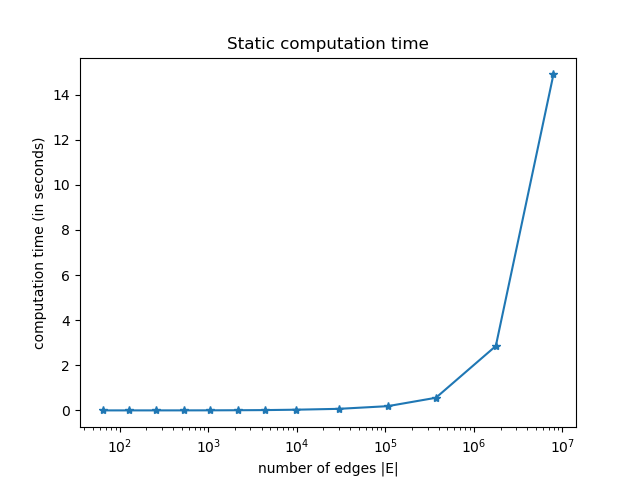
\includegraphics[width=0.48\textwidth]{static.png}
 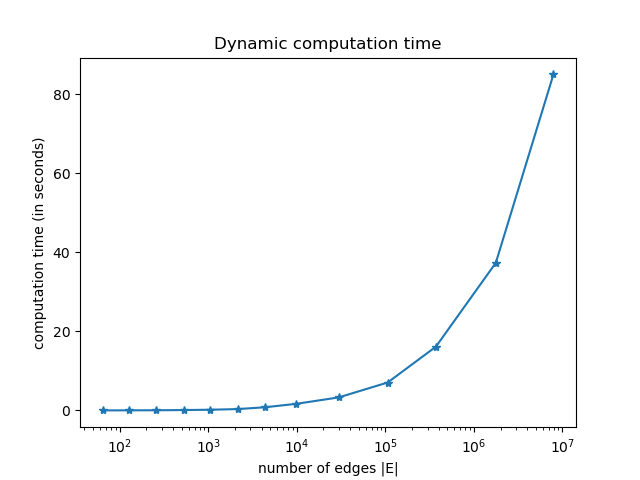
\includegraphics[width=0.48\textwidth]{dynamic.png}
\end{tcolorbox}

\end{itemize}



\subsection{Deliverables}\label{subsec:deliv}
\begin{itemize}
\item code for initial, static MST implementation
\item code for dynamic MST recomputation
\item README, explaining how to run your code
\item Report (Subsection \ref{subsec:report})
\item output files (13) within the $results$ folder- one for each graph
\end{itemize}


\begin{thebibliography}{100}
 \bibitem{rmat}  D. Chakrabarti, Y. Zhan, and C. Faloutsos. R-MAT: A Recursive Model for Graph Mining. In \emph{Proc. 4th SIAM Intl. Conf. on Data Mining,} Florida, USA, April 2004.



\end{thebibliography}

\end{document}
